\section{Einführung in das Projekt}
\label{sec:intro}

Im Rahmen des Projekts implementieren die Student\_innen\footnote{Diese Schreibweise wird durchg\"angig verwendet, um alle m\"oglichen Personen gleichberechtigt anzusprechen, auch wenn sie
f\"ur den\_die Leser\_in vielleicht teilweise irritierend wirkt. Betrachten Sie dies als Reflektionsm\"oglichkeit! Mehr Informationen unter 
\url{http://de.wikipedia.org/wiki/Geschlechtergerechte_Sprache\#Sichtbarmachung} bei \glqq{}Gender Gap\grqq{}.}
in Gruppen von jeweils vier Personen eine Java-Version des Spiels \emph{\gameTitle.} Die Aufgabenstellung stellt zun\"achst das zugrundeliegende Spiel vor.

Die Aufgabe kann in vier verschiedenen \glqq Ausbaustufen\grqq\ bearbeitet werden, die jeweils eine unterschiedliche Punktzahl zur Gesamtnote beitragen. Die minimale Ausbaustufe muss zum Erreichen der Mindestpunktzahl \textbf{vollst\"andig} implementiert werden.

Ab Ausbaustufe I können nicht erreichte Punkte der gegebenen Ausbaustufe durch Elemente h\"oherer Ausbaustufen \glqq{}ausgeglichen\grqq{} werden. Projektabgaben, die \glqq{}zwischen\grqq{} Ausbaustufen liegen, bei denen also erwartete Inhalte fehlen oder zusätzliche Elemente eingebaut wurden, sind natürlich ebenfalls möglich; die Ausbaustufen geben nur eine grobe Orientierung vor. Beachten Sie dabei jedoch, dass die Ausbaustufen nach Schwierigkeitsgrad gruppiert sind, d.h.  Aufgaben h\"oherer Stufen sind in der Regel schwieriger zu l\"osen als Aufgabenteile niedrigerer Ausbaustufen.

%\newpage
\subsection{Das Spiel \emph{\gameTitle}}
 ////////////////ändern! gameIntro.tey
Im Spiel \emph{\gameTitle{}} spielen Sie Eins gegen Eins. Jede Person steuert dabei einen Gorilla und versucht den gegnerischen Gorilla mit einer Banane abzuwerfen. Die Gorillas stehen in gewisser Entfernung, einer links und einer rechts, auf verschiedenen Hochh\"ausern einer Skyline. Das Spiel ist rundenbasiert: Zun\"achst t\"atigt der/die erste Spieler\_in den Wurf. Trifft dieser Wurf, so wurde die Runde gewonnen, ansonsten ist der/die n\"achste Spieler\_in an der Reihe. Ein Wurf wird durch zwei Eingaben gesteuert: den Abwurfwinkel und die Wurfgeschwindigkeit. Der Winkel wird als Gradzahl von 0 bis 360 angegeben, die Geschwindigkeit auf einer Skala von 0 bis 200.

Abbildung \vref{fig:screenshot1} zeigt ein m\"ogliches Menü. Abbildung \vref{fig:screenshot2} zeigt ein mögliches Spielfenster. Wir erwarten nicht, dass 
das im Rahmen des Projekts erstellte Spiel der Ausgabe optisch \"ahnlich sieht; die 
Abbildung soll nur zum besseren Nachvollziehen dienen.

Auf einem beliebig großen rechteckigen Spielfeld kann es folgende Spielobjekte geben:
\begin{description}
\item[Gorilla]
Jeder Spieler verfügt über einen Gorilla. Folglich befinden sich zum Start zwei Gorillas, einer links und einer rechts, auf dem Feld. Gorillas unterschiedlicher Parteien müssen nicht visuell unterscheidbar sein.
\item[Hochhaus]
Die Gorillas stehen auf Hochhäusern, die eine Skyline bilden.
\item[Banane]
Tätigt ein Spieler einen Wurf, so fliegt eine Banane (hoffentlich) in Richtung des gegnerischen Gorillas.
\end{description}

\begin{figure}[htb]
\begin{center}
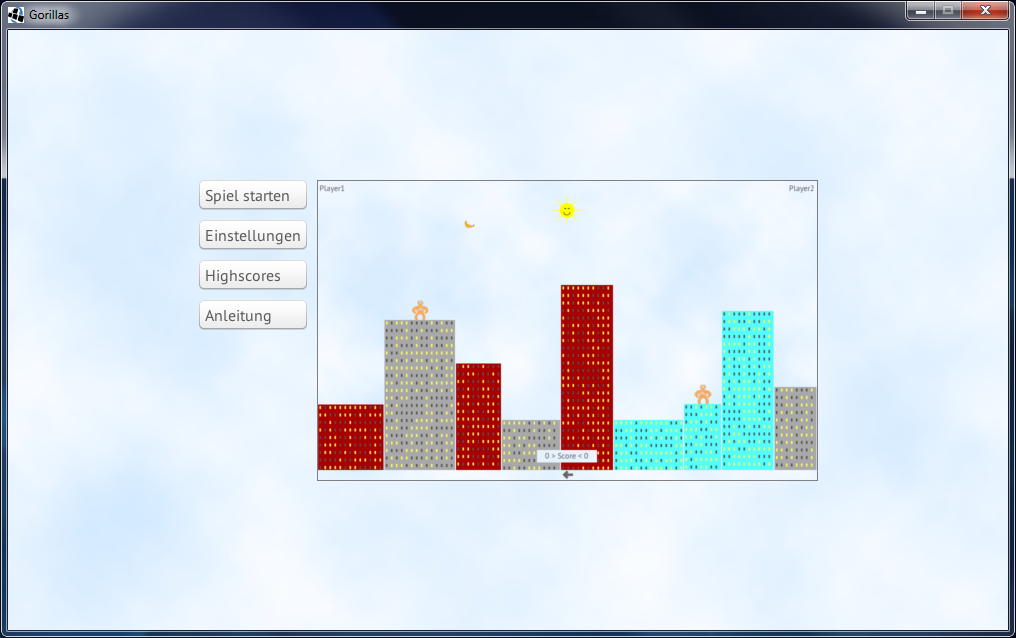
\includegraphics[scale=0.4]{\basepath/\shortGameTitle/menu.png}
\caption{Beispiel einer grafischen Umsetzung des Menüs von \gameTitle}
\label{fig:screenshot1}
\end{center}
\end{figure}

\begin{figure}[htb]
\begin{center}
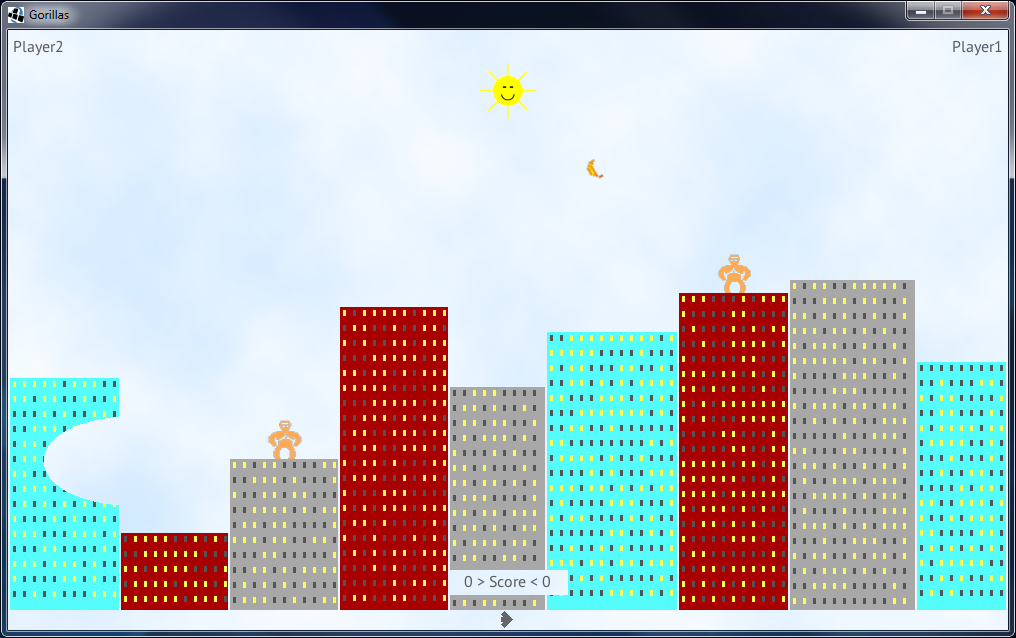
\includegraphics[scale=.4]{\basepath/\shortGameTitle/gameplay.png}
\caption{Beispiel einer grafischen Umsetzung des Spielfensters von \gameTitle}
\label{fig:screenshot2}
\end{center}
\end{figure}
